As a result of the analysis conducted during the screening rounds, this section addresses the proposed research questions.

\subsection{RQ1: What are the challenges of integrating quantum computing systems with an existing classical computing infrastructure?}

The integration of hybrid quantum/classical systems presents several challenges, which can be categorized into four main areas: scalability and performance, data and encoding, algorithm and software development, and developers' expertise.

\noindent\textbf{Scalability and performance}

Scalability involves the system's capacity to expand, while performance relates to meeting time/resources constraints efficiently. Although limited research addresses these attributes in quantum software, running the mapping methodology consolidates relevant findings. According to \cite{Elsharkawy2023}, key scaling challenges include supporting diverse quantum technologies, managing high latency, and addressing the lack of standardization in programming languages and service providers. \cite{Cerezo2022, Sodhi2021} discuss the exponential increase in quantum noise as solutions scale. Additionally, \cite{Sodhi2021} highlights hardware limitations affecting software resilience, and \cite{Vietz2021} points out performance issues related to queue times for quantum services.

\noindent\textbf{Data and encoding}

Encoding classical data into quantum states is a significant challenge. M. Cerezo and Daniel Vietz \cite{Cerezo2022, Vietz2021} both emphasize the difficulty in defining the boundary between quantum and classical systems. Furthermore, \cite{Cerezo2022} notes the scarcity of high-quality, standardized datasets for quantum systems which complicates benchmarking optimization algorithms and training AI models.

\noindent\textbf{Algorithmic and software development}

Quantum software development often requires unique algorithms for each problem, limiting the reuse of existing components and hardware \cite{Moguel2022, Sodhi2021}. \cite{Moguel2022, Vietz2021} highlight the lack of standardization among quantum providers as a development challenge, while \cite{40} points to the absence of observability tools. An additional challenge is simulating quantum systems on classical hardware, particularly calculating inner products, as discussed in \cite{Cerezo2022}. The authors also identify finding local minima of loss functions in quantum systems as an NP-hard problem, which is no different from existing classical solutions.

\noindent\textbf{Developers' expertise}

The developers' expertise is being discussed as one of the major challenges of quantum computing, since it requires a low-level knowledge to solve problems \cite{Moguel2022, De_Maio_Kanatbekova_Zilk_Friis_Guggemos_Brandic_2024}. A reality today is that having expertise in the quantum domain is not enough to develop quantum solutions, since programmers should also need to know about software integration, service-oriented architectures, cloud computing and workflow development \cite{Vietz2021, Sodhi2021, De_Maio_Kanatbekova_Zilk_Friis_Guggemos_Brandic_2024}. Finally, as simulation is a required step, and resources are limited in local development environments, developers need to use remote machines to test the algorithms, thus complicating the coding experience \cite{Sodhi2021}.

\subsection{RQ2: What attributes and/or metrics of classical software quality are relevant to the quantum realm, and which are unique in the context of quantum computing?}

The response to this research question is structured in two distinct sections: the first examines quality attributes, while the second explores quality metrics.

\noindent\textbf{Quality attributes}

Our review enabled us to evidence that the challenges of quantum systems are expressed in terms of attributes well-known in the software community.

%\textit{scheduling}, which ensures single tasks do not block access to resources \cite{Elsharkawy2023}, and 

%And \textit{data management}, focusing on efficient coordination between quantum and classical systems \cite{Elsharkawy2023}, are also crucial infrastructure considerations.
%\textit{Latency}, measured as the time elapsed for a single task \cite{Elsharkawy2023},

From a developmental perspective, \textit{scalability}, which refers to the system's capacity to increase available resources \cite{Elsharkawy2023}, \textit{understandability} is essential, determining how easily developers can comprehend the created code \cite{Elsharkawy2023}. \textit{Functional suitability} measures the degree to which developers can trust the results \cite{Wang2023}, \cite{Faryal2022}, \cite{30}, while \textit{performance efficiency} addresses speed and resource utilization \cite{Wang2023} \cite{Elsharkawy2023}, \cite{Faryal2022}, \cite{30}. \textit{Usability} focuses on the ease of using quantum tools \cite{Wang2023}, \cite{Faryal2022}, \cite{30}, and \textit{reliability} measures the code's ability to handle errors effectively \cite{Wang2023}, \cite{Faryal2022}, \cite{30}.

\textit{Security} aspects are addressed through the code's capacity to manage undesired behavior \cite{Wang2023}, \cite{Faryal2022}, \cite{30}, while \textit{maintainability} reflects how easily software can be repaired \cite{Wang2023}, \cite{Faryal2022}, \cite{30}. The quality of technology documentation is captured in \textit{user documentation} attributes \cite{Wang2023}. Finally, system integration attributes include \textit{portability}, which measures the ease of running software on different hardware \cite{Faryal2022}, \cite{30}, and \textit{compatibility}, which reflects the ability of two components to interact on the same hardware \cite{Faryal2022}, \cite{30}.

\noindent\textbf{Quality metrics}

As was the case for the attributes, the review allowed us to identify that popular metrics from classical computing are used in quantum computing. In addition, the research revealed metrics specifically unique to quantum computing. These measurements, especially those concerning hardware characteristics and circuit behavior, have been adapted for evaluating quantum software quality. The identified metrics include:

Hardware quality metrics focus on evaluating quantum computers, including measurements such as T1 (Energy relaxation, "\textit{the time needed for a qubit to move from the excited state $\ket{1}$ to the ground state $\ket{0}$} \cite{youssefMeasuringSimulatingT12020}") and T2 (Dephasing, "\textit{the elapsed time before a qubit's resonance frequency becomes unidentified} \cite{youssefMeasuringSimulatingT12020}") \cite{Alam2019}. System reliability is assessed through error measurements, particularly the percentage of failures on gates \cite{Alam2019}.

Performance-related metrics evaluate how efficiently the code solves tasks; measured through quantum volume and total quantum factor \cite{Verduro2021}. \textit{Precision} examines how close measurements are to each other \cite{Moguel2022}, while \textit{accuracy} determines how close responses are to the true value \cite{Verduro2021}. \textit{Decoherence}, representing information lost due to environmental factors \cite{Verduro2021}, and response times between request and result \cite{Moguel2022} are crucial operational metrics.

Maintainability metrics include the economic cost of quantum infrastructure \cite{Moguel2022} and the complexity of gate operations, which measures the number of Qubits, Gates, and Oracles used \cite{Moguel2022, 40, Díaz_Alvarado-Valiente_Romero-Álvarez_Moguel_Garcia-Alonso_Rodríguez_García-Rodríguez_Murillo_2025}. Circuit density evaluates the quantity of gates applied to each qubit at specific circuit steps \cite{26}. Additionally, Oracle-related measurements focus on unexposed operations used as input to other quantum algorithms \cite{26}.

Quantum circuit complexity can be evaluated based on structural metrics identified in \cite{Díaz_Alvarado-Valiente_Romero-Álvarez_Moguel_Garcia-Alonso_Rodríguez_García-Rodríguez_Murillo_2025}: \textit{Circuit Width (CW)} measures the total number of qubits in a circuit, while \textit{Circuit Depth (CD)} represents the longest path from input to output. The \textit{Complexity of circuit gates (CCG)} evaluates the intricacy of gate operations, and \textit{Conditional instructions (CI)} quantifies the number of classical control operations. \textit{Quantum cyclomatic complexity (QCC)} provides a measure of the program's structural complexity. Additional operational metrics include \textit{Measurement operations (MO)}, counting the number of quantum measurements, \textit{Initialize and reset operations (IRO)} tracking system resets, and \textit{Auxiliary qubits (AQ)} measuring the number of additional qubits required for computation.

\subsection{RQ3: In how many studies are the RQ1 and RQ2 explicitly addressed?}

The analysis of the 16 selected articles revealed an interesting distribution in the coverage of our research questions. Regarding RQ1, 7 studies explicitly addressed the challenges of quantum-classical integration, representing 43\% of the total sample. In contrast, RQ2 received substantially more attention, with 14 articles (87\%) discussing quality metrics and attributes in quantum computing systems.

This distribution highlights a significant research gap in the mapping study of hybrid systems. Such disparity is not unexpected, considering the early stage of quantum computing technology and the inherent complexity of integration issues. The predominant focus on quality metrics and attributes suggests that the research community is primarily concerned with establishing fundamental quality standards and evaluation frameworks, which is crucial for the field's maturation.

\begin{figure}
\begin{center}
\begin{minipage}{0.48\textwidth}
    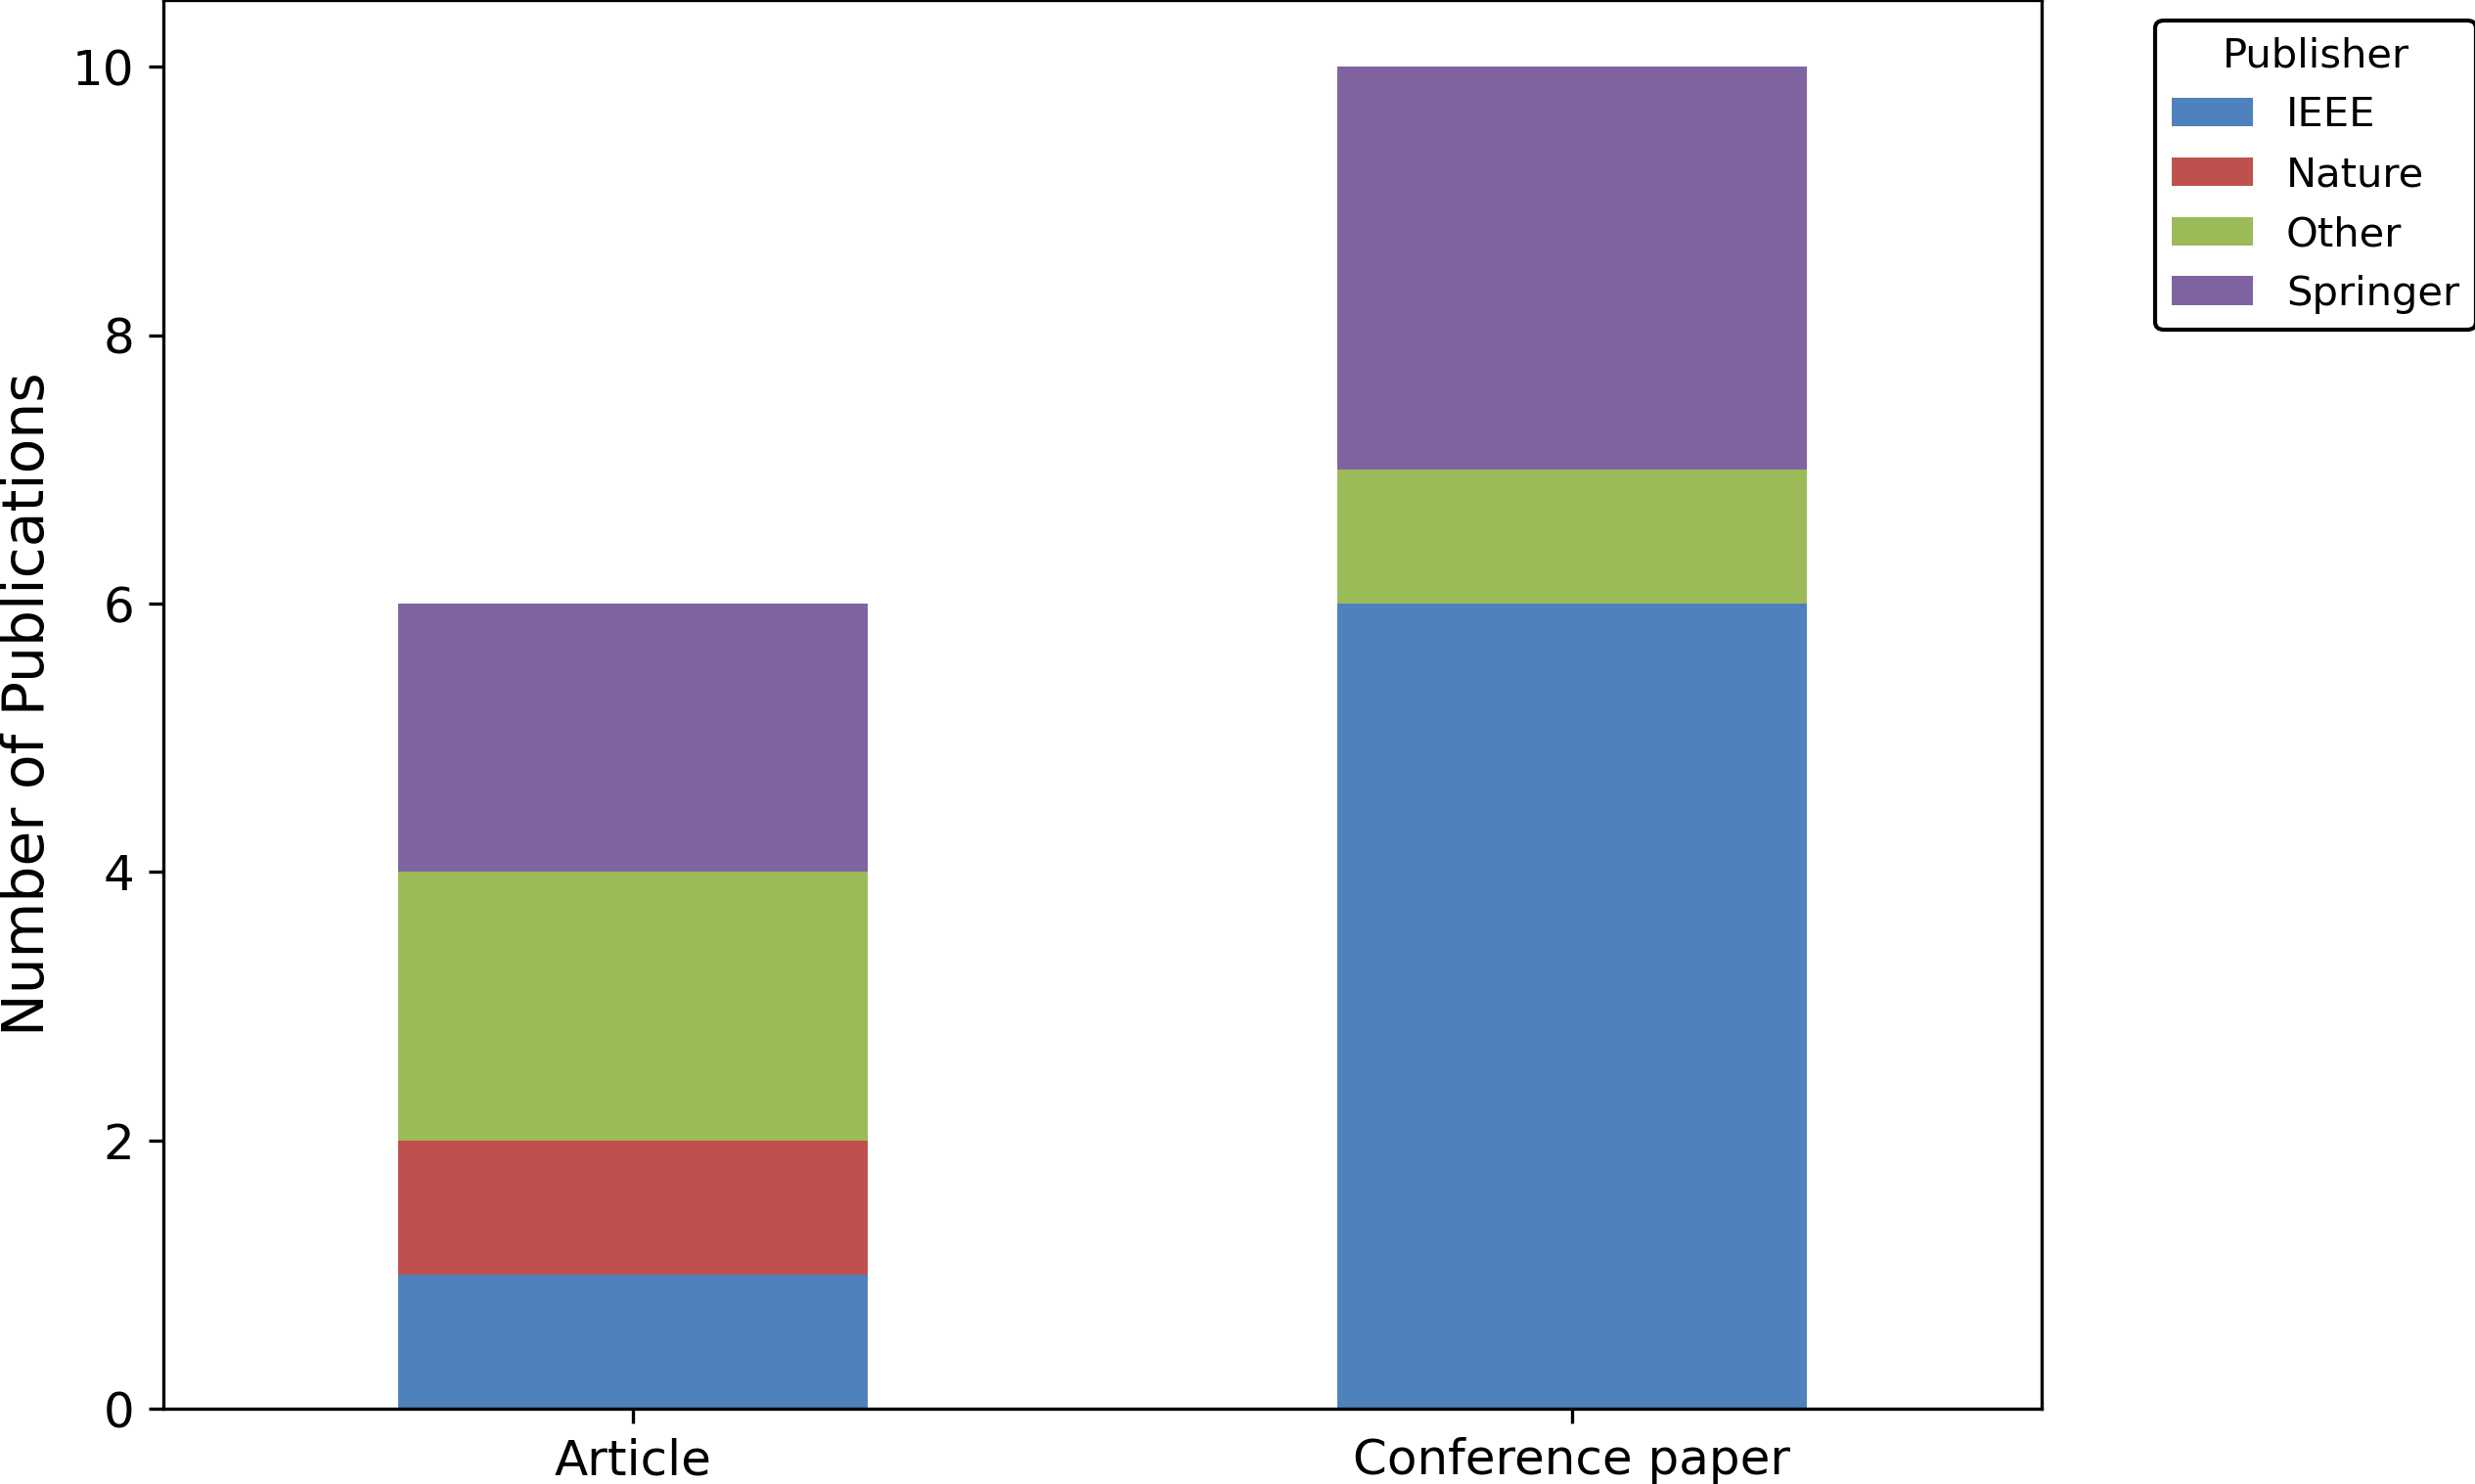
\includegraphics[width=\textwidth]{photo/conf_by_editor.png}
    \caption{Distribution of publication types across publishing entities.}
    \label{fig:studies_type_per_year}
\end{minipage}
\hfill
\begin{minipage}{0.48\textwidth}
    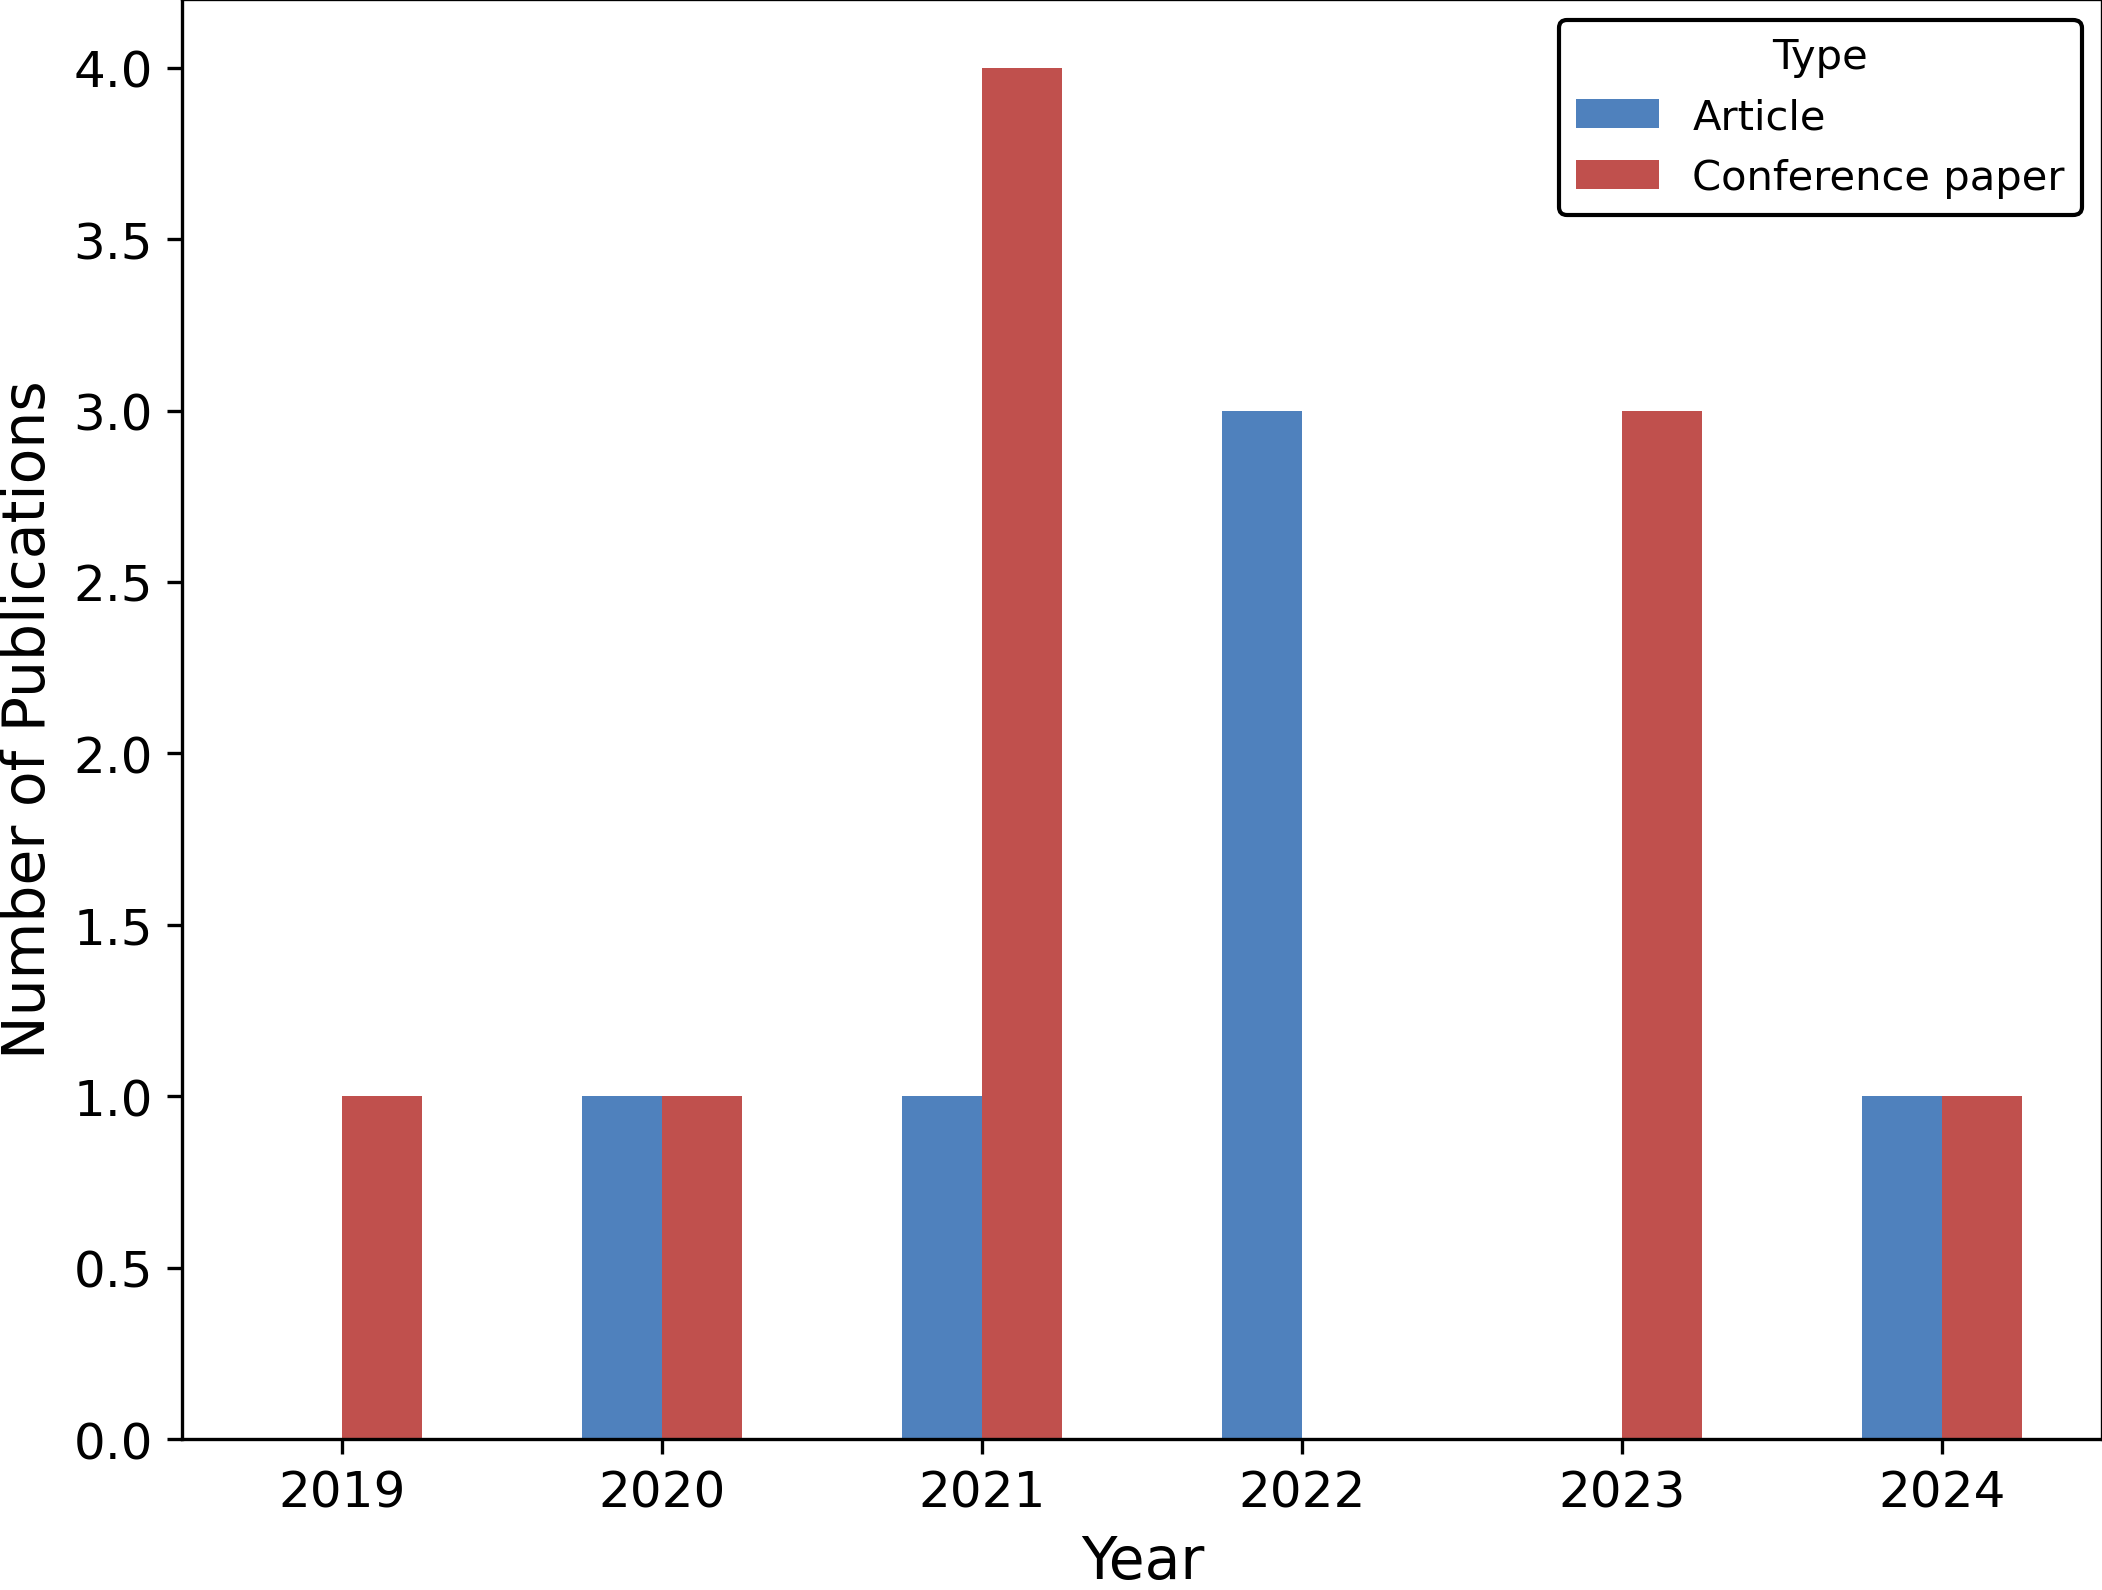
\includegraphics[width=\textwidth]{photo/by_year.png}
    \caption{Temporal distribution of publication types.}
    \label{fig:studie_type_per_year}
\end{minipage}
\end{center}
\end{figure}

\subsection{RQ4: What are the types of research and contributions of the selected studies? }

The systematic mapping study revealed that the majority of the selected literature consists of conference proceedings (62\%, n=10), with the remaining publications appearing in peer-reviewed journals (37\%, n=6). The conference papers were predominantly presented at IEEE-sponsored events and Springer communications, while the journal articles were distributed across prestigious publications including Nature, Springer, ACM, and IEEE journals.

Figure \ref{fig:studies_type_per_year} illustrates the distribution of publication types across different publishers. The analysis reveals a notable concentration of conference papers affiliated with IEEE, suggesting its significant role in facilitating early-stage quantum computing research discussions. However, the journal publications demonstrate a more diverse distribution across publishers, with no single entity emerging as the dominant platform for quantum computing quality attribute research. This distribution pattern may reflect the emerging nature of the field, where rapid dissemination through conferences currently takes precedence over longer-format journal publications.

\subsection{Q5: What is the publication year, the type of publication, and the research group that contributed to answering RQ1 and RQ2? }

The temporal analysis of publications, as illustrated in Figure \ref{fig:studie_type_per_year}, reveals a consistent pattern in the distribution of research outputs. Conference proceedings dominated the publication landscape across all years examined, with the notable exception of 2022. This prevalence of conference publications can be attributed to several factors: the rapid evolution of quantum computing research necessitating swift dissemination of findings, the preliminary nature of many studies in this emerging field, and the value of conference venues for fostering immediate discourse within the research community.
